\documentclass{article}

\usepackage[spanish]{babel}
\usepackage{titling}
\usepackage{graphicx}
\usepackage{graphicx}
\usepackage[export]{adjustbox}
\usepackage{hyperref}
\usepackage{ragged2e}
\usepackage{indentfirst}
\usepackage{float}
\usepackage{microtype}
\usepackage[bottom]{footmisc}
\usepackage{fancyhdr}
\fancyhead[R]{2020}\fancyhead[L]{UNC - FCEFyN} \fancyfoot[C]{\thepage}
\pagestyle{fancy}

%%%%%%%%%%%%%%%%%%%%%%%%%%%%%%%%%%%%%%%%%%%%%%%%%%%%%%%%%%%%%%%%%%%%%%%%%%%%%%%

\title{Universidad Nacional de Córdoba\\Facultad de Ciencias Exactas, Físicas y Naturales}
\author{Tomas Sarquis}
\date{Diciembre 2020}

%%%%%%%%%%%%%%%%%%%%%%%%%%%%%%%%%%%%%%%%%%%%%%%%%%%%%%%%%%%%%%%%%%%%%%%%%%%%%%%

\hypersetup{
    colorlinks,
    citecolor=black,
    filecolor=black,
    linkcolor=blue,
    urlcolor=black
}

%%%%%%%%%%%%%%%%%%%%%%%%%%%%%%%%%%%%%%%%%%%%%%%%%%%%%%%%%%%%%%%%%%%%%%%%%%%%%%%

\newcommand{ \fnintelydrone }{\footnote{\url{www.intelydrone.com}}}
\newcommand{ \fnincubadora }{\footnote{\url{www.incubadoradeempresas.unc.edu.ar}}}
\newcommand{ \fntrace }{\footnote{\url{www.intelydrone.com/root/latest/products.html}}}
\newcommand{ \fnarduino }{\footnote{\url{www.arduino.cc}}}
\newcommand{ \fnfreertos }{\footnote{\url{www.freertos.org}}}
\newcommand{ \fnespressif }{\footnote{\url{www.espressif.com}}}
\newcommand{ \fnesp }{\footnote{\url{www.espressif.com/en/products/modules/esp32}}}
\newcommand{ \fnidosc }{\footnote{\url{docs.espressif.com/projects/esp-idf/en/latest/esp32/api-reference/peripherals/i2c.html}}}
\newcommand{ \fnmasterslave }{\footnote{\url{en.wikipedia.org/wiki/Master/slave_(technology)}}}
\newcommand{ \fnidoscdevlib }{\footnote{\url{www.github.com/jrowberg/i2cdevlib}}}
\newcommand{ \fnmodulo }{\footnote{En las pruebas realizadas, éste valor no supera las 100 unidades}}
\newcommand{ \fnstackof }{\footnote{\url{www.stackoverflow.com/questions/63780850/esp32-best-way-to-store-data-frequently}}}
\newcommand{ \fnnvs }{\footnote{\url{docs.espressif.com/projects/esp-idf/en/latest/esp32/api-reference/storage/nvs_flash.html}}}
\newcommand{ \fnwifi }{\footnote{El sistema debía usar \emph{LoRa} pero el estudiante no contó con el \emph{hardware} necesario}}
\newcommand{ \fnsleep }{\footnote{El estudio del consumo considera únicamente las etapas de \emph{sleep} ya que en ésta etapa transcurre más del 90\% del programa}}
\newcommand{ \fnejemplos }{\footnote{\url{www.github.com/espressif/esp-idf/tree/master/examples/system/deep_sleep}}}
\newcommand{ \fnrepo }{\footnote{\url{www.github.com/tsarquis88/esp32_freertos}}}

%%%%%%%%%%%%%%%%%%%%%%%%%%%%%%%%%%%%%%%%%%%%%%%%%%%%%%%%%%%%%%%%%%%%%%%%%%%%%%%

\begin{document}

%%%%%%%%%%%%%%%%%%%%%%%%%%%%%%%%%%%%%%%%%%%%%%%%%%%%%%%%%%%%%%%%%%%%%%%%%%%%%%%

    \begin{titlingpage}
        \maketitle
        \null \null \null \null 
        
        \begin{center}
            {\huge Práctica Supervisada}
        \end{center}
        
        \topskip0pt % (?)
        
        \null \null \null \null \null \null 
        
        \begin{center}
            {\large \textbf{Monitoreo del movimiento de animales vacunos}}
        \end{center}
        
        \begin{center}
            {\large \textbf{Supervisor}: Gustavo Wolfmann }
        \end{center}

    \end{titlingpage}

%%%%%%%%%%%%%%%%%%%%%%%%%%%%%%%%%%%%%%%%%%%%%%%%%%%%%%%%%%%%%%%%%%%%%%%%%%%%%%%

    \tableofcontents 

%%%%%%%%%%%%%%%%%%%%%%%%%%%%%%%%%%%%%%%%%%%%%%%%%%%%%%%%%%%%%%%%%%%%%%%%%%%%%%%

    \newpage
    \section{Introducción}

    El presente documento detalla la realización de la práctica profesional
    supervisada llevada a cabo por el estudiante Tomas Sarquis, perteneciente 
    a la carrera de Ingeniería en Computación. \par

    La práctica fue realizada para \emph{Intelydrone}\fnintelydrone, empresa 
    que actualmente se encuentra radicada en la encubadora de empresas de la 
    Universidad Nacional de Córdoba\fnincubadora, y que se desempeña en el 
    rubro de \emph{Innovación Tecnológica en Ganaderia}. Gustavo Wolfmann,
    supervisor de la práctica que éste documento detalla, forma parte del 
    equipo fundador de \emph{Intelydrone}. \par

    El trabajo realizado tuvo que ver con uno de los productos que la empresa
    ofrece: el \emph{Intelytrace}. Este ``es un dispositivo de posicionamiento 
    y seguimiento que es colocado en cada animal en forma de collar en su 
    cuello.``\fntrace 

    \begin{figure}[h]
        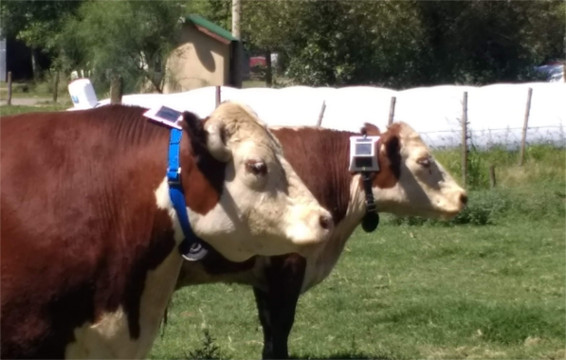
\includegraphics[width=0.7 \textwidth, center]{../primeras/trace.jpg}
        \caption{Vacas con el \emph{Intelytrace} en sus cuellos}
        \label{fig:trace}
    \end{figure} 

    \par
    El \emph{Intelytrace} tiene varias funcionalidades, sin embargo, la 
    práctica supervisada se centró en el monitorio del movimiento de los 
    animales. \par

    La práctica profesional tuvo una duración de 200 (doscientas) horas, 
    repartidas en 41 (cuarenta y  uno) días.

%%%%%%%%%%%%%%%%%%%%%%%%%%%%%%%%%%%%%%%%%%%%%%%%%%%%%%%%%%%%%%%%%%%%%%%%%%%%%%%
    
    \newpage
    \section{Entorno de trabajo}

    \subsection{Propuesta}
    Si bien Intelydrone ya contaba con un sistema que cumplía con la tarea 
    de monitoreo de movimiento, la empresa buscaba rehacer el mismo, ya que el
    existente no cumplía con ciertos aspectos que se deseaban mejorar. Entre 
    éstos últimos, se encontraban el poco ahorro de energía (cuestión muy 
    importante debido a que el sistema funciona en una placa embebida 
    alimentada por batería) y el hecho de que el programa en la placa estaba
    desarrollado con librerías de \emph{Arduino}\fnarduino. \par

    Debido a lo anterior, se le propuso al alumno llevar a cabo la tarea 
    anteriormente mencionada cumpliendo los siguientes requisitos:

    \begin{itemize}
        \item El programa debe ejecutarse bajo el sistema operativo de tiempo
        real \emph{FreeRTOS}\fnfreertos.
        \item El programa debe estar implementado en el lenguaje de 
        programación \emph{C++}.
        \item El sistema debe ser corrido en la placa \emph{ESP32}\fnesp de 
        \emph{Espressif}\fnespressif.
        \item El sistema debe ahorrar el máximo de energía posible.
    \end{itemize}
    
    \subsection{Lugar de trabajo}
    La práctica profesional se llevó a cabo en un contexto de cuarentena causada 
    por la pandemia mundial del año 2020. Es por esto que el alumno realizó la 
    labor en su domicilio, previamente habiéndose puesto de acuerdo con su 
    supervisor y proporcionándole, éste último, del \emph{hardware} necesario 
    para comenzar a trabajar. Para otras consultas laborales, se recurrió a 
    medios de comunicación virtuales.

    \subsection{Hardware}
    El \emph{hardware} utilizado para llevar a cabo el sistema consta de dos 
    partes importantes: el módulo \emph{ESP32-WROOM} (figura \ref{fig:esp32})
    y el sensor \emph{MPU6050} (figura \ref{fig:mpu}). Siendo esta última, 
    un módulo que funciona como acelerómetro, termómetro y/o giroscópio. \par

    Además, para llevar a cabo el diseño de la manera más cómoda posible, se
    utilizó el \emph{ESP32-DevKit}.

    \begin{figure}[h]
        \includegraphics[width=0.6 \textwidth, center]{../primeras/esp32.png}
        \caption{Módulo (izquierda) y \emph{DevKit} (derecha)}
        \label{fig:esp32}
    \end{figure} 

    \begin{figure}[h]
        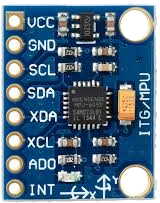
\includegraphics[width=0.3 \textwidth, center]{../primeras/mpu.png}
        \caption{Sensor de movimiento}
        \label{fig:mpu}
    \end{figure} 

%%%%%%%%%%%%%%%%%%%%%%%%%%%%%%%%%%%%%%%%%%%%%%%%%%%%%%%%%%%%%%%%%%%%%%%%%%%%%%%

    \newpage
    \section{Descripción del trabajo}   

    \subsection{Investigación}
    Las primeras horas de trabajo fueron dedicadas a la familiarización del 
    \emph{hardware}: se le instaló el sistema operativo y se le dieron tareas
    simples para probar su correcto funcionamiento. \par
    El paso siguiente fue el de leer la \emph{API Guide} de \emph{Espressif}, 
    con la cual el estudiante pudo conocer las funciones proveídas por los 
    desarrolladores oficiales y conocer el alcance de las mismas. Dichas 
    funciones son usadas constantemente en el programa, y sin ellas la 
    implementación sería mucho más ardua. \par
    Posteriormente, la documentación del sensor también fue estudiada, ya que 
    uno debe conocer los registros internos y sus distintas maneras de 
    funcionamiento. \par
    Se pudo, además, acceder a la documentación de la primera implementación
    del sistema (recordar que \emph{Intelydrone} ya contaba con el mismo, pero 
    se buscaba mejorar). De esta forma, el estudiante adquirió una idea clara 
    del producto final. \newline \par

    La etapa de investigación, que duró 10 (diez) días, sirvió para tener un 
    mejor entendimiento general de la labor, y así poder encarar de forma 
    óptima la etapa de desarrollo. \par
    Cabe aclarar que el estudiante se enconcontró en situaciones de 
    investigaciones posteriores, a pesar de haber terminado la etapa.

    \subsection{Desarrollo}
    Una vez familiarizado con los dispositivo (\emph{ESP32} y \emph{MPU6050}),
    lo primero que se hizo fue armar el circuito de pruebas (figura 
    \ref{fig:circuito}) para poder empezar a tomar las primeras medidas de 
    aceleración. Dicho circuito se utilizó para el desarrollo únicamente, ya 
    que más adelante se iba a utilizar la placa integrada del \emph{Intelytrace}.
    \par
    En las siguientes subsecciones, se detalla el desarrollo de las partes 
    principales del sistema en orden cronológico.

    \begin{figure}[h]
        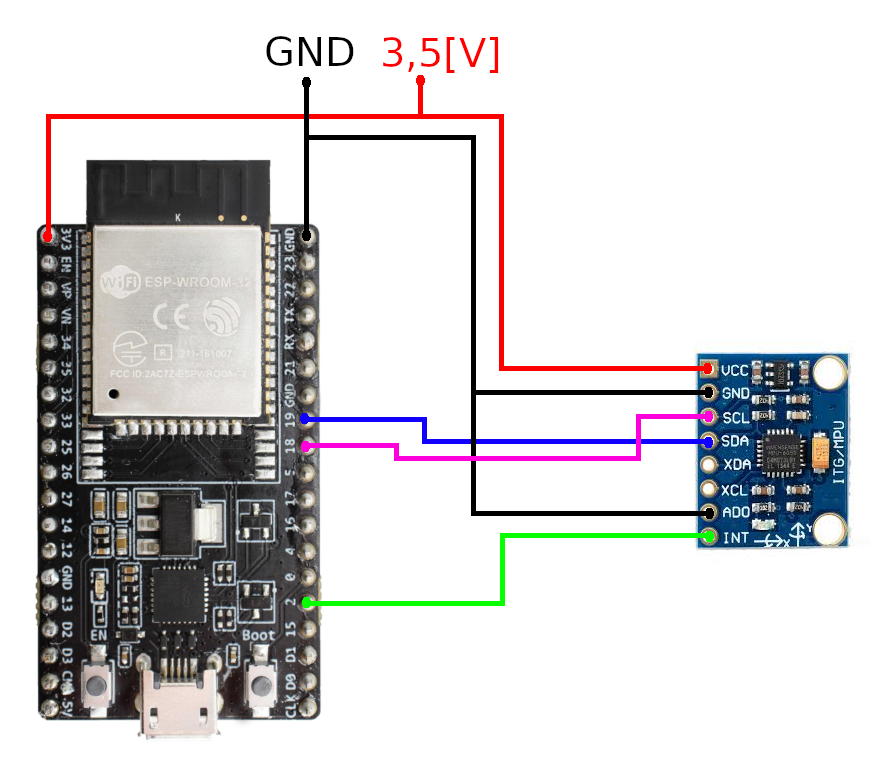
\includegraphics[width=0.9 \textwidth, center]{../primeras/circuito.png}
        \caption{Circuito de pruebas}
        \label{fig:circuito}
    \end{figure}

    \subsubsection{Comunicación serie}
    Debe existir una constante comunicación entre el micro y el sensor, tanto 
    para la configuración del útlimo, como para la recepción de las mediciones.
    Para esto, el sensor es compatible con el protocolo de comunicación serie
    \emph{I2C}\fnidosc, que utliza el modelo de control \emph{master/slave}
    \fnmasterslave. \par
    Para la configuración del \emph{driver} se utilizan las funciones de los
    fabricantes, mientras que para el uso del \emph{bus}, o sea, envío y 
    recepción de datos, se usa la librería \emph{i2cdevlib}, de \emph{jrowberg}
    \fnidoscdevlib.

    \subsubsection{Configuración del sensor}
    Cuando el programa bootea (inicia por primera vez), lo primero que se hace
    es configurar el sensor para poder empezar a utilizarlo. Como se dijo 
    anteriormente, esto se realiza mediante una comunicación serie, en la cual
    se leen y/o escriben registros del sensor. \par
    Algunas de las configuraciones hechas, que se consideran importantes, son:
    \begin{itemize}
        \item \textbf{Activación de FIFO:} Se activa una cola, del tipo
        \emph{FIFO}, de 1024 bytes para almacenar mediciones.
        \item \textbf{Interrupciones:} Se avisa al micro, mediante una 
        interrupción, que la cola del sensor se ha llenado. Mientras el sensor
        va llenando la cola, el micro ahorra energía, y cuando la cola se llena,
        el micro ``despierta`` y la vacía.
        \item \textbf{Apagado de sensores:} Se apagan el sensor giroscópico y 
        el de temperatura, ya que no son tenidos en cuenta.
        \item \textbf{Calibración:} Se calibra el sensor, de forma que, cuando
        se encuentra quieto, las mediciones arrojen un valor cercano al cero.
        \item \textbf{Arranque de mediciones:} En su estado inicial el sensor
        no realiza mediciones, por lo que se lo debe configurar para que 
        empiece a hacerlo.
    \end{itemize}

    \subsubsection{Recepción de mediciones}
    A medida que el sensor va tomando mediciones, los valores de las mismas
    van escribiéndose en la cola \emph{FIFO}. La estructura y el orden de lo 
    anterior se refleja en la tabla \ref{tab:registros}. \par

    \begin{table}[h]
        \centering
        \begin{tabular}{||c||} 
            \hline
            Registro \\ [0.5ex] 
            \hline\hline
            ACCEL\_XOUT\_H\_0 \\ 
            \hline
            ACCEL\_XOUT\_L\_0 \\ 
            \hline
            ACCEL\_YOUT\_H\_0 \\ 
            \hline
            ACCEL\_YOUT\_L\_0 \\ 
            \hline
            ACCEL\_ZOUT\_H\_0 \\ 
            \hline
            ACCEL\_ZOUT\_L\_0 \\ 
            \hline
            ACCEL\_XOUT\_H\_1 \\ 
            \hline
            ACCEL\_XOUT\_L\_1 \\ 
            \hline
            ACCEL\_YOUT\_H\_1 \\ 
            \hline
            ACCEL\_YOUT\_L\_1 \\ 
            \hline
            ACCEL\_ZOUT\_H\_1 \\ 
            \hline
            ACCEL\_ZOUT\_L\_1 \\ 
            \hline
            ... \\ 
            \hline
            ACCEL\_XOUT\_H\_N \\ 
            \hline
            ACCEL\_XOUT\_L\_N \\ 
            \hline
            ACCEL\_YOUT\_H\_N \\ 
            \hline
            ACCEL\_YOUT\_L\_N \\ 
            \hline
            ACCEL\_ZOUT\_H\_N \\ 
            \hline
            ACCEL\_ZOUT\_L\_N \\ 
            \hline
        \end{tabular}
        \caption{Estructura de cola con mediciones registradas, siendo \emph{N} la 
        cantidad de las mismas}
        \label{tab:registros}
    \end{table}

    Una medición consiste en 3 valores: uno por cada eje gravitacional (X,Y,Z).
    Los valores de cada eje tienen un largo de 16 \emph{bits}, que son guardados
    en 2 registros de 8 \emph{bits} cada uno, lo que da un total de 6 registros 
    por medición (un total de 48 \emph{bits}). Lo que interesa es saber el 
    módulo del vector gravitacional, que es calculado como:
    
    \[ |ACCEL| = \sqrt{ ACCEL\_OUT\_X^2 + ACCEL\_OUT\_Y^2 + ACCEL\_OUT\_Z^2 } \]

    Finalmente, el módulo es mapeado a un valor entero de 8 \emph{bits}, que 
    puede ir desde 0 (mínima aceleración) a 255 (máxima aceleración)\fnmodulo.
    
    \subsubsection{Primeras mediciones obtenidas}
    Los primeros resultados arrojados se pueden observar en la figura 
    \ref{fig:resultados_devkit}, los cuales fueron obtenidos midiendo la 
    aceleración humana caminando y trotando a distintas velocidades. La 
    cantidad de mediciones es de 506.

    \begin{figure}[H]
        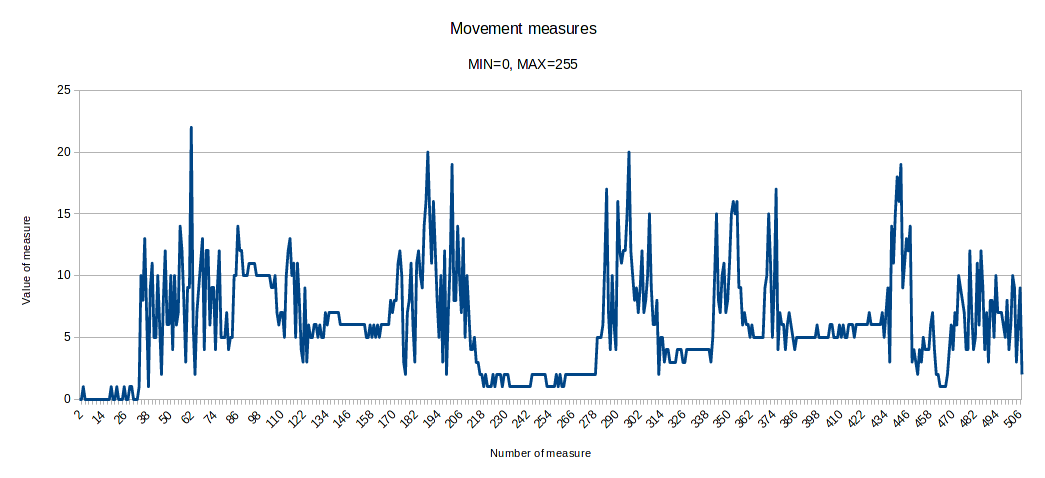
\includegraphics[width=1.0 \textwidth, center]{../primeras/results_devkit.png}
        \caption{Primeras mediciones obtenidas}
        \label{fig:resultados_devkit}
    \end{figure}

    \subsubsection{Almacenamiento}
    El microcontrolador cuenta con distintas maneras de almacenar datos. \par
    Primeramente se optó por utilizar la memoria \emph{NVS}\fnnvs 
    (``Almacenamiento no volátil``) por su facilidad, pero se tuvo que pensar 
    en otra manera debido a que este método utliza la memoria \emph{Flash}, y 
    el uso constante de la misma tiende a degradarla. \par
    Finalmente, con ayuda del supervisor de práctica, se decidió por usar un 
    sistema (figura \ref{fig:memoria}) de memorias de dos niveles: los datos 
    recibidos desde el sensor se van acumulando en la memoria \emph{RTC RAM} 
    del microcontrolador (que no se degrada con el uso), y cuando ésta se 
    llena, se transfieren los datos al \emph{filesystem SPIFFS} (que tiene 
    muchas más capacidad de almacenamiento), dejando vacía la primera. 
    Luego se vuelve a usar la \emph{RTC RAM}, y el proceso se repite hasta 
    que el \emph{filesystem} agota su capacidad. \par
    El sistema \emph{SPIFFS} utliza la memoria \emph{Flash}, pero como está
    en un ``segundo nivel``, no se escribe tan seguido y por lo tanto, no 
    se degrada tan rápidamente. \par
    Cuando el \emph{filesystem} se llena, se debe vaciar y transferir los
    datos al servidor. \par
    Se busca que el envío de las mediciones no se realice de manera frecuente, 
    ya que el consumo de energía se vería afectado negativamente. Es por esto
    que se intentó aprovechar al máximo la fase de almacenamiento.

    \begin{figure}[h]
        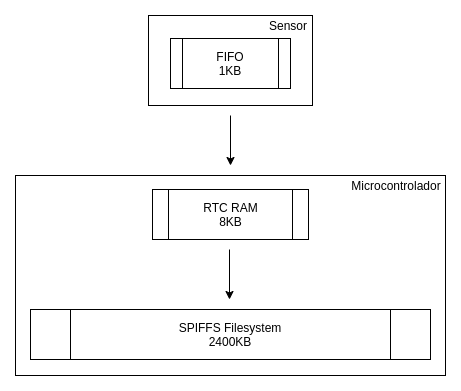
\includegraphics[width=0.8 \textwidth, center]{../segundas/esquema_memoria.png}
        \caption{Esquema de memoria en niveles}
        \label{fig:memoria}
    \end{figure}

    \subsubsection{Transferencia}
    La idea es que, cuando sea necesario, se pueda enviar todas las mediciones
    a un servidor de la red local (en un \emph{drone} que circula cerca) de 
    forma segura. Para esto, se usó el protocolo \emph{HTTP}, mientras que 
    la tecnología inalámbrica fue \emph{Wi-Fi}\fnwifi. \par
    La transferencia consiste en varios paquetes \emph{HTTP} de tamaño 
    configurable. Para las pruebas se han usado paquetes de 100 datos cada uno.

    \begin{figure}[h]
        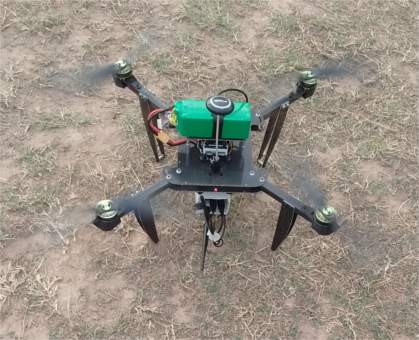
\includegraphics[width=0.8 \textwidth, center]{../segundas/drone.jpg}
        \caption{\emph{Drone} funcionando como servidor}
        \label{fig:drone}
    \end{figure}

    \subsubsection{FreeRTOS}
    El sistema operativo que orquesta el sistema es \emph{FreeRTOS}, el cuál
    estuvo diseñado por 3 tareas:
    \begin{itemize}
        \item \textbf{Tarea principal:} Encargada de crear las demás tareas y 
        los recursos compartidos.
        \item \textbf{Tarea de acelerómetro:} Su misión es la de recepción y 
        almacenamiento de las mediciones.
        \item \textbf{Tarea de transferencia:} Realiza las tareas de envío
        de datos al servidor.
    \end{itemize}

    \subsection{Resultados}
    Los resultados a continuación detallados han sido recavados de la ejecución
    del sistema en el \emph{Intelytrace} y no en la placa de pruebas.

    \subsubsection{Mediciones}
    Los resultados arrojados se pueden observar en la figura 
    \ref{fig:resultados_modulo}, los cuales fueron obtenidos midiendo la 
    aceleración humana caminando y trotando a distintas velocidades. La 
    cantidad de mediciones es de 1488.

    \begin{figure}[h]
        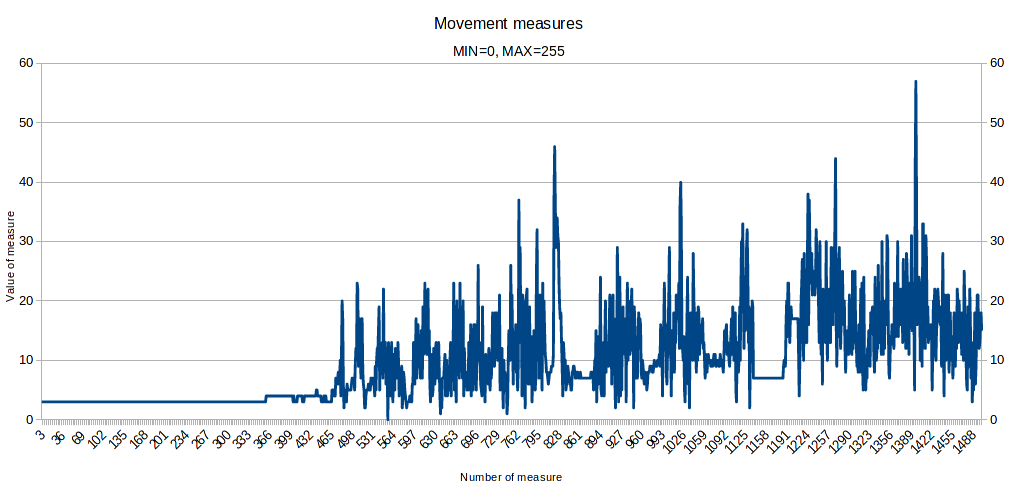
\includegraphics[width=1.0 \textwidth, center]{../segundas/results_module.png}
        \caption{Resultados obtenidos}
        \label{fig:resultados_modulo}
    \end{figure}

    \subsubsection{Consumo}
    Uno de los requisitos principales era que el consumo de la placa sea lo 
    menor posible y para esto se hizo incapié en que el microcontrolador se 
    encuentre en modo \emph{sleep} la mayor parte del tiempo.\fnsleep \par
    A pesar de esto, los resultados obtenidos en cuanto al amperaje no fueron
    los esperados, como se puede ver en la tabla \ref{tab:consumo}. \par
    Cabe aclarar que la corriente eléctrica (consumo) fue medida en serie
    a la batería que alimenta toda la placa.

    \begin{table}[h]
        \centering
        \begin{tabular}{||c|c||} 
            \hline
            Consumo esperado & Consumo obtenido \\ [0.5ex] 
            \hline\hline
            10 [uA] & 4.3 [mA] \\
            \hline
        \end{tabular}
        \caption{Consumo esperado y obtenido (\emph{deep-sleep mode})}
        \label{tab:consumo}
    \end{table}

    Si bien no se sabe, a ciencia cierta, a qué se debe esta diferencia de 
    consumo, la misma no se atribuye a un problema del \emph{software} 
    implementado, ya que se han llevado a cabo pruebas con programas 
    oficiales\fnejemplos y los resultados han sido los mismos. \par
    Por su parte, la placa incrustada en el \emph{Intelytrace} no solo cuenta 
    con el ESP32, si no que cuenta, además, con otros componentes de 
    \emph{hardware} como cargador de batería, receptor LoRa WAN y GPS, por lo 
    que se plantea como hipótesis que dichos componentes sean los causantes del 
    alto consumo, y no el ESP32 propiamente dicho.

%%%%%%%%%%%%%%%%%%%%%%%%%%%%%%%%%%%%%%%%%%%%%%%%%%%%%%%%%%%%%%%%%%%%%%%%%%%%%%%

    \newpage
    \section{Conclusión}

    La práctica supervisada ha sido una actividad realmente enriquecedora tanto
    para el alumno como para el supervisor y su empresa. El estudiante tuvo una
    experiencia real de la implementación completa de un \emph{software}, 
    pasando por el análisis de los requerimientos, el diseño, las posibilidades
    de desarrollo, las investigaciones posteriores y finalmente el desarrollo y
    los resultados. \par
    El sistema implementado en estos meses es susceptible a (y debería, en lo 
    posible) ser mejorado, ya que ciertas cuestiones del programa lo ameritan.
    Además, se recomienda hacer más pruebas de \emph{testing}, ya que el 
    desarrollador pudo hacer solamente las pruebas básicas. \par
    Algunas mejoras podrían ser:
    \begin{itemize}
        \item Reemplazar la conexión WiFi por LoRa WAN
        \item Tener en cuenta valores de movimiento relativos. Esto es, no solo
        tener en cuenta los valores absolutos, si no, además, computar las 
        diferencias de movimiento en función del tiempo. Esto podría ser útil
        para detectar cambios bruscos de movimiento.
        \item Arreglo de \emph{bugs}
    \end{itemize} \par
    A pesar de esto y teniendo en cuenta el tiempo empleado para el desarrollo 
    y la poca experiencia del desarrollador, el resultado es muy favorable: los
    requerimientos fundamentales han sido satisfechos. \par
    Los conocimientos obtenidos en la universidad y las ayudas recibidas por
    parte del supervisor y de la comunidad informática, fueron de necesidad para
    el estudiante.

%%%%%%%%%%%%%%%%%%%%%%%%%%%%%%%%%%%%%%%%%%%%%%%%%%%%%%%%%%%%%%%%%%%%%%%%%%%%%%%

\newpage
\section{Apéndice}

El código del programa implementado se puede apreciar en el repositorio\fnrepo 
del desarrollador. Los archivos de interés se encuentran
sobre el directorio \emph{esp-idf/main} que, a su vez, contiene tres 
directorios más:
\begin{itemize}
    \item \emph{include}. Contiene los \emph{headers} del código fuente.
    \item \emph{lib}. Dentro se encuentran las librerías externas que han sido 
    usadas.
    \item \emph{src}. El código fuente de cada tarea se encuentra aquí.
\end{itemize} \par
El área de mayor interés es, quizás, la del directorio \emph{src}. En él se 
encuentran implementadas las tareas del sistema, por lo que para conocer su
funcionamiento, es de crucial importancia entender estos códigos.

%%%%%%%%%%%%%%%%%%%%%%%%%%%%%%%%%%%%%%%%%%%%%%%%%%%%%%%%%%%%%%%%%%%%%%%%%%%%%%%

\end{document}